\chapter{Einstein-Proca equations of motion}
\label{appendixb}



As an illustrative example, we provide here explicit expressions for the equations of motion solved by KBHsPH. The components of the Einstein tensor for the ansatz~\eqref{eqn:HBH-ansatz} are:

\begin{eqnarray}
&&  4r^2  e^{2F_1}{\bf G_{tt}}= 4 
N \left[r^2 ({F_1}_{,rr}+ {F_2}_{,r}^2+
{F_2}_{,rr})
+r( 
{F_1}_{,r}+3  {F_2}_{,r})+1\right] + 2 r N'  \left(r 
{F_1}_{,r}+r {F_2}_{,r}+2\right)+4 {F_1}_{,\theta\theta}\nonumber \\
%
&& +4  
{F_2}_{,\theta}^2+4  {F_2}_{,\theta\theta}
%
+8
\cot \theta {F_2}_{,\theta}-4 
%
 +r^4 \sin ^2\theta e^{2 ({F_2}-F_0)} 
 \left\{
 \frac{2W W_{,r}}{r}(- r {F_0}_{,r} +3r{F_2}_{,r}+4 )
 +W_{,r}^2+2W W_{,rr} 
 \right. \nonumber \\ 
%
&& \left. + \frac{2 W \left[W_{,\theta} \left(- 
{F_0}_{,\theta}+3 {F_2}_{,\theta}+3 \cot\theta\right)+ W_{,\theta\theta}\right]+ W_{,\theta}^2}{r^2N} \right\},
\end{eqnarray}

\begin{equation}
\frac{2Ne^{2(F_0+F_1-F_2)}}{\sin^2\theta}{\bf G_{t\phi }}=   W_{,\theta} \left[ {F_0}_{,\theta}-3 \left( 
{F_2}_{,\theta}+\cot\theta\right)\right]- \left\{r N 
\left[W_{,r} \left(-r {F_0}_{,r}+3 r 
{F_2}_{,r}+4\right)+r 
W_{,rr}\right]+W_{,\theta\theta}\right\}  ,
\end{equation}



\begin{eqnarray}
&&  \frac{e^{2F_1}}{N}{\bf G_{rr}}= \frac{({F_0}_{,\theta}+\cot\theta)({F_0}_{,\theta}-{F_1}_{,\theta}+
{F_2}_{,\theta})+{F_2}_{,\theta}({F_2}_{,\theta}-{F_1}_{,\theta})
+{F_0}_{,\theta\theta}+{F_2}_{,\theta\theta}-1+[Nr]'}{r^2 N}+{F_1}_{,r} {F_2}_{,r}\nonumber \\
&& 
%2{F_0}_{,r} +{F_1}_{,r}+{F_2}_{,r}
%
+\frac{2{F_0}_{,r}+{F_1}_{,r}+{F_2}_{,r}}{r}(1+r)+\frac{e^{2(
{F_2}- {F_0})} \sin ^2\theta (r^2W_{,r}^2N-W_{,\theta}^2 ) }{4 N^2} 
%
+\frac{N'( 
{F_1}_{,r}+{F_2}_{,r})}{2N},
\end{eqnarray}


\begin{eqnarray}
 && e^{2F_1}r^2{\bf G_{r\theta}}=
 %
\cot\theta (
{F_1}_{,r} -{F_2}_{,r} )-{F_0}_{,r\theta}-{F_2}_{,r\theta}+\frac{{F_0}_{,\theta}+{F_1}_{,\theta}}{r}+\frac{r^2 \sin ^2\theta 
W_{,\theta} W_{,r} e^{2( {F_2}- {F_0})}-N'( {F_0}_{,\theta}-{F_1}_{,\theta})}{2 
N} \nonumber \\ 
&& + {F_0}_{,r} ({F_1}_{,\theta}-{F_0}_{,\theta})+
{F_1}_{,r}({F_0}_{,\theta}+{F_2}_{,\theta} )+{F_2}_{,r}( {F_1}_{,\theta}- {F_2}_{,\theta} ),
\end{eqnarray}




\begin{eqnarray}
&&  e^{2F_1}r^2{\bf G_{\theta\theta}}=r^2 N\left[ {F_0}_{,r}({F_0}_{,r}- 
{F_1}_{,r}+{F_2}_{,r}) + {F_0}_{,rr}+
{F_2}_{,rr}+ {F_2}_{,r}^2-{F_1}_{,r} {F_2}_{,r} \right]
%
+{F_0}_{,\theta}( {F_1}_{,\theta}+ 
{F_2}_{,\theta})
%
 \nonumber \\
&&
+{F_1}_{,\theta} \
{F_2}_{,\theta}
+\cot \theta( {F_0}_{,\theta}+ {F_1}_{,\theta})+\frac{r^2 \sin ^2\theta 
 e^{2( {F_2}- {F_0})}\left(W_{,\theta}^2-Nr^2  W_{,r}^2\right)}{4 N}+r^2 N' \left(\frac{3}{2} {F_0}_{,r}-\frac{1}{2}  {F_1}_{,r}+
{F_2}_{,r}+\frac{1}{r}\right)
 \nonumber \\
&&
+\frac{1}{2} r^2 \
N''
+r N(
{F_0}_{,r}-
{F_1}_{,r}+2 {F_2}_{,r}),
\end{eqnarray}



\begin{eqnarray}
&& 4r^2e^{2F_1}{\bf G_{\phi\phi}}= 2 r N'  \left(3 r {F_0}_{,r}+r 
{F_1}_{,r}+2\right)+4 (
{F_0}_{,\theta}^2  +4{F_0}_{,\theta\theta}+ {F_1}_{,\theta\theta}) +2 r^2 N''  \nonumber \\
%
&& 
%
+4 r N  \left[r \left({F_0}_{,rr}+{F_1}_{,rr}\right)+r 
{F_0}_{,r}^2+{F_0}_{,r}+{F_1}_{,r}\right] +r^4 \sin ^2\theta e^{2 ({F_2}-F_0)}\left\{ W W_{,r}\left(2  {F_0}_{,r}-6 {F_2}_{,r}-\frac{8}{r}\right)-3  W_{,r}^2\right. \nonumber \\
%
&&
\left.-2 WW_{,rr}- \frac{\left\{2 W \left[W_{,\theta} \left(- {F_0}_{,\theta}
+3 {F_2}_{,\theta}+3 \cot \theta\right)+ W_{,\theta\theta}\right]+3 W_{,\theta}^2\right\}}{Nr^2}\right\} .
\end{eqnarray}






The components of the Proca energy-momentum tensor~\eqref{procaemt}, for the ansatz~\eqref{procaclouds} and the geometry~\eqref{eqn:HBH-ansatz} are also involved because of the four extra functions in the Proca ansatz, and the three new parameters $m,w,\mu$; but they can still be presented in a fairly compact form:

\begin{eqnarray}
&& 2e^{2F_0+2F_1+2F_2}{\bf T_{tt}}=e^{2F_2}\left[ W^2(m{H_1}  
- \sin\theta  
{H_3}_{,r} )^2
-(wH_1+V_{,r})^2\right] \nonumber \\
% 
&&
-\frac{N e^{2 ({F_0}-F_1)}}{r^2} \left\{e^{2 {F_1}}\left[ {\mu^2} r^2 {H_1}^2 e^{2 {F_2}}
+({m} \csc \theta  {H_1}
-{H_3}_{,r})^2\right] +e^{2
{F_2}}\left( {H_1}_{,\theta}- 
{H_2}_{,r}\right)^2\right\}
\nonumber \\
%
&&
- \frac{e^{2 F_0}}{r^4} \left[{\mu^2} 
r^2( {H_3}^2 e^{2 {F_1}}+ {H_2}^2 e^{2
{F_2}}) + ({H_3}_{,\theta}+ \cot
\theta  {H_3}-mH_2\csc\theta)^2\right]  \nonumber \\
%
%
&&
+\frac{ e^{2 (F_1+{F_2})} {\mu^2} r^2\left({H_3}^2  W^2 \sin ^2\theta  - V^2\right) -e^{2 {F_1}}\left(
{m} \csc\theta 
 V +w{H_3}  \right)^2 }{r^2N} \nonumber \\
 &&
 +\frac{ e^{2 {F_2}}\left\{W^2[(H_3\sin\theta)_{,\theta}-mH_2]^2-[V_{,\theta}+wH_2]^2\right\}}{r^2N}, \nonumber \\
 && 
%
%\left[{H_3} \cos \theta+\sin \theta  {H_3}_{,\theta} \right]^2-2 {H_2} 
%\left({m} \sin \theta {H_3}_{,\theta} W^2+{m} \cos\theta 
%{H_3} W^2+w V_{,\theta}\right)- 
%{H_2}^2 \left(w^2-{m}^2 W^2\right)- 
%V_{,\theta}^2\right]\right\} \nonumber
\end{eqnarray}


\begin{eqnarray}
&&  e^{2F_0+2F_1}{\bf T_{t\phi}}=\frac{[mH_2-(\sin\theta H_3)_{,\theta}][V_{,\theta}+W(H_3\sin\theta)_{,\theta}}{r^2N} \nonumber\\
&& +\frac{H_2(w-mW)]-{\mu^2}r^2 \sin\theta {H_3} e^{2 {F_1}} \left[ 
V+WH_3 \sin\theta\right]}{r^2N}\nonumber \\ 
%
&&
- \left({m} {H_1}-\sin\theta 
{H_3}_{,r}\right) \left[{H_1} ({m} W-w)-\sin \theta {H_3}_{,r} W-V_{,r}\right],
\end{eqnarray}






\begin{eqnarray}
&& 2r^4e^{2(F_0+F_1+F_2)}{\bf T_{rr}}=
r^2 N e^{2 {F_0}} \left[
e^{2 F_2} {H_1}^2 {\mu^2} r^2
+\left( {m H_1} \csc\theta- {H_3}_{,r}\right)^2+e^{2 ({F_2}-F_1)}( {H_1}_{,\theta}-
{H_2}_{,r})^2\right] \nonumber \\ 
%
&&
-{\mu^2} r^2e^{2 {F_0}}( {H_3}^2 e^{2 {F_1}}+{H_2}^2e^{2F_2})-e^{2 {F_0}}\csc\theta\left[(\sin\theta{H_3})_{,\theta}-mH_2\right]^2  \nonumber \\
%
&&
-r^4 e^{2 {F_2}} \left[ {H_1} (w-{m} W) + \sin\theta  {H_3}_{,r} W+  
V_{,r}\right]^2 \\
%
%
%
&&
+\frac{r^2}{N} \left\{e^{2 {F_1}}({m} \csc\theta 
 V+{H_3}w)^2 +{\mu^2} r^2e^{2 ({F_1}+F_2)}[V+ {H_3} W \sin\theta]^2 
 \right. \nonumber \\
&& \left.
+e^{2 {F_2}}\left[
V_{,\theta}+ (\sin\theta  
{H_3})_{,\theta} W+ 
{H_2} (w-{m} W)\right]^2\right\},
%
\end{eqnarray}





\begin{eqnarray}
&&  r^2e^{2F_1}{\bf T_{r\theta}}= \frac{ \csc ^2\theta e^{-2 {F_2}}}{r^2} \left({m} {H_1}-\sin \theta {H_3}_{,r}\right) 
 \left[{m} {H_2}-(\sin\theta 
{H_3})_{,\theta}\right] +{\mu^2}  {H_1} 
{H_2}
 \nonumber \\
%
&&
+\frac{e^{-2 {F_0}}}{N} \left\{[ (w-{m}W) {H_1}+V_{,r}+ W{H_3}_{,r}\sin\theta ] \left[(w-{m}W) {H_2}+V_{,\theta}+W
(\sin\theta{H_3})_{,\theta}\right]
\right\},
\end{eqnarray}









\begin{eqnarray}
&& 2r^4e^{2(F_0+F_1+F_2)}{\bf T_{\theta\theta}}=-r^2 N e^{2 {F_0}} \left[e^{2 F_2} {H_1}^2 
{\mu^2} r^2 +( m\csc\theta H_1-{H_3}_{,r})^2  -e^{2( {F_2}-F_1)}( {H_1}_{,\theta}- 
{H_2}_{,r})^2\right] \nonumber \\
%
&&
-{\mu^2} r^2e^{2 {F_0}}({H_3}^2 e^{2 {F_1}}-{H_2}^2e^{F_2})
+e^{2 {F_0}} \left(\cot \theta {H_3}-m{H_2} \csc\theta+ {H_3}_{,\theta}\right)^2
 \nonumber \\
%
&&
+ r^4 e^{2 {F_2}} \left[
 {H_1} (w-{m} W)+ \sin\theta  {H_3}_{,r} W+
V_{,r} \right]^2 \nonumber \\
&&
%
+\frac{r^2}{N} \left\{e^{2 {F_1}}({m} \csc\theta 
 V+{H_3}w)^2 +{\mu^2} r^2e^{2 ({F_1}+F_2)}[V+ {H_3} W \sin\theta]^2 
 \right. \nonumber \\
%
&&
\left.
-e^{2 {F_2}}\left[
V_{,\theta}+ (\sin\theta  
{H_3})_{,\theta} W+ 
{H_2} (w-{m} W)\right]^2\right\},
\end{eqnarray}









  %%%%%%%%%%%%%%%%%

 \begin{eqnarray}
&& 2e^{2F_0+2F_1+2F_2}{\bf T_{\phi\phi}}=e^{2F_2}\left[ -W^2(m{H_1}  
- \sin\theta  
{H_3}_{,r} )^2
+(wH_1+V_{,r})^2\right] \nonumber \\
% 
&&
-\frac{N e^{2 {F_0}}}{r^2} \left\{\left[ {\mu^2} r^2 {H_1}^2 e^{2 {F_2}}
-({m} \csc \theta  {H_1}
-{H_3}_{,r})^2\right] +e^{2(
{F_2}-F_1)}\left( {H_1}_{,\theta}- 
{H_2}_{,r}\right)^2\right\}
\nonumber \\
%
&&
+ \frac{e^{2 F_0}}{r^4} \left[{\mu^2} 
r^2( {H_3}^2 e^{2 {F_1}}- {H_2}^2 e^{2
{F_2}}) + ({H_3}_{,\theta}+ \cot
\theta  {H_3}-mH_2\csc\theta)^2\right]  \nonumber \\
%
%
&&
+\frac{- e^{2 (F_1+{F_2})} {\mu^2} r^2\left({H_3}^2  W^2 \sin ^2\theta  - V^2\right) -e^{2 {F_1}}\left(
{m} \csc\theta 
 V +w{H_3}  \right)^2}{r^2N} \nonumber \\
 && \frac{-e^{2 {F_2}}\left\{W^2[(H_3\sin\theta)_{,\theta}-mH_2]^2-[V_{,\theta}+wH_2]^2\right\}}{r^2N} .
\nonumber \\
 && 
\end{eqnarray}  
  %%%%%%%%%%%%%%%%%%



The four  Proca potentials satisfy the equations\footnote{In deriving this form, we have used
the Proca field equations~\eqref{procafe} together with the Lorentz condition (\ref{lorentz}).}:
\begin{eqnarray}
&&
( r^2 N'-2rN)  W( mH_1
- \sin \theta   {H_3}_{,r} )
-r^2 w N'  {H_1}+\frac{e^{2( {F_1}-F_0)}}{N} V \left[r^2 
(w-{m} W)^2
 \right. \nonumber \\
%
&&
\left.
-N e^{2 {F_0}} 
\left({\mu^2} r^2 +{m}^2 \csc 
^2\theta e^{-2F_2}\right)\right]
+[2 (\sin \theta {H_3})_{,\theta} W+V_{,\theta}-2mWH_2)] 
(-{F_0}_{,\theta}+{F_2}_{,\theta}+\cot\theta) 
 \nonumber \\
%
&&
+(\sin \theta  {H_3})_{,\theta} W_{,\theta}
+ V_{,\theta\theta}
+r N  \left\{
 [2 W(mH_1- \sin \theta   {H_3}_{,r})-V_{,r}] \left(r {F_0}_{,r}-r 
{F_2}_{,r}\right)
-rH_1 \left(2 w {F_0}_{,r}+{m} 
W_{,r}\right)
 \right. \nonumber \\
%
&&
\left.
+r \sin \theta {H_3}_{,r} W_{,r}+2 
V_{,r}+r V_{,rr}\right\}
+r^2 \sin ^2\theta e^{2 ({F_2}-F_0)}
W\left\{
 W_{,\theta} \frac{\left[{H_2} (w-{m} W)+(\sin \theta
{H_3})_{,\theta} W+V_{,\theta}\right]}{N}
 \right. \nonumber \\
%
&&
\left.
+r^2 W_{,r}[
H_1(w-{m}  W) 
+ \sin\theta  {H_3}_{,r} W
+ V_{,r} ]
\right\}
-{H_2} 
\left[
2 w {F_0}_{,\theta}+{m} W_{,\theta}\right] 
=0, \nonumber \\
&&
\end{eqnarray}


\begin{eqnarray}
&&  r^3 [{H_1} N]'' + r^2 [{H_1} N]'  \left(r {F_0}_{,r}-2 r {F_1}_{,r}+r 
{F_2}_{,r}+2\right)
-r N  {H_1} \left[2 r {F_1}_{,r} \left(r 
{F_0}_{,r}+r {F_2}_{,r}+2\right)
 \right. \nonumber \\
%
&&
\left.
-r^2( 
{F_0}_{,rr}+ {F_2}_{,rr})+2\right]
+[r {H_1}_{,\theta}-2 {H_2}\left(r {F_1}_{,r}+1\right)] ( {F_0}_{,\theta}+ {F_2}_{,\theta}+\cot\theta ) \nonumber \\
%
&&
+rH_2( {F_0}_{,r\theta}+
 {F_2}_{,r\theta})
 -r {H_1}e^{2 {F_1}} \left({\mu^2} r^2 +e^{-2F_2}{m}^2 \csc ^2\theta\right)
   \nonumber \\
%
&&
%-2 r {F_1}_{,\theta} {H_1}_{,\theta}
-2( r {F_1}_{,r}+1) {H_2}_{,\theta}
+2 r {F_1}_{,\theta} ({H_2}_{,r} -{H_1}_{,\theta})
+r  {H_1}_{,\theta\theta} 
+2 {m}  \csc\theta e^{2 
({F_1}-F_2)}{H_3} (r {F_2}_{,r}+1) 
%
 \nonumber \\
%
&&
+\frac{r^3  e^{2 
({F_1}-F_0)}}{N} \left\{
\left(2{F_0}_{,r}+\frac{N'}{N}\right)(w-mW)(V+\sin \theta {H_3} 
W )
 \right. \nonumber \\
%
&&
\left.
+W_{,r}[ \sin \theta {H_3}  
(W {m}-w)+m(V+\sin\theta H_3W)] 
\right\} =0, \nonumber \\
&&
\end{eqnarray}


 %%%%%%%%%%%%%%%%%%%%%%%%%%%%%%% 

\begin{eqnarray}   
&& 
r^2 [N {H_2}_{,r}]'
-2 r^2 {F_1}_{,\theta} [N{H_1}]'
+{H_2}_{,\theta\theta}
+ {H_2}_{,\theta} \left({F_0}_{,\theta}-2 {F_1}_{,\theta}+{F_2}_{,\theta}+\cot\theta\right)
\nonumber \\
%
&&
+2 {m} \csc \theta e^{2 ({F_1}-F_2)} {H_3} \left({F_2}_{,\theta}
+\cot \theta\right) 
+r^2 N {H_2}_{,r} \left[{F_0}_{,r} 
-2 {F_1}_{,r} 
+{F_2}_{,r} \right]
\nonumber \\
%
&&
-rN{H_1} \left[2 {F_1}_{,\theta} \left(r {F_0}_{,r}+r {F_2}_{,r}+2\right) 
-r \left({F_0}_{,r\theta}+{F_2}_{,r\theta}\right)\right]
+2rN \left(r {F_1}_{,r}+1\right) {H_1}_{,\theta}
\nonumber \\
%
&&
- H_2 \left[2 {F_1}_{,\theta} 
\left({F_0}_{,\theta}+{F_2}_{,\theta}+\cot \theta\right)
-{F_0}_{,\theta\theta} +{\mu^2} r^2 e^{2 
{F_1}}+{m}^2 \csc ^2\theta e^{2( 
{F_1}-F_2)}- {F_2}_{,\theta\theta}+\csc ^2\theta \right] \nonumber \\
%
&&
+\frac{r^2 e^{2 ({F_1}-F_0)} }{N}
\left\{ {H_2} (w-{m} W)^2 
 \right. \nonumber \\
%
&&
\left.
+2{F_0}_{,\theta}(w-mW)(V+\sin\theta H_3W)+W_{,\theta}[\sin \theta {H_3}(Wm-w)+m(V+\sin \theta {H_3}W)]\right\} =0,  \nonumber \\
&&
\end{eqnarray}




\begin{eqnarray}
&&
r^2 [N  {H_3}_{,r}]'
+{H_3}_{,\theta\theta}+ {H_3} 
 \left[
  \cot \theta ({F_0}_{,\theta} -{F_2}_{,\theta})
 - {\mu^2} r^2 e^{2 {F_1}}
 - {m}^2 \csc ^2\theta e^{2( 
{F_1}-F_2)}
-\csc ^2\theta 
\right] 
  \nonumber \\
%
&&
+{H_3}_{,\theta} \left({F_0}_{,\theta}-{F_2}_{,\theta}+\cot \theta\right)
+\sin\theta r^4e^{2 ({F_2}-F_0)}W_{,r}[
   {H_1}(m W 
- w)   
-( \sin \theta  {H_3}_{,r} W 
+ V_{,r}) ]
  \nonumber \\
%
&&
+2 {m} \csc \theta [
{H_2} 
\left({F_2}_{,\theta}+\cot \theta\right) 
+ rN 
\left(r {F_2}_{,r}+1\right) {H_1}]
+ r^2N{H_3}_{,r} \left({F_0}_{,r} 
-{F_2}_{,r}\right)
+\frac{ r^2e^{-2F_0} }{N} 
\left\{
{H_3}e^{2 {F_1}} \left({m}  W-w \right)^2 
 \right. \nonumber \\
%
&&
\left.
- e^{2 {F_2}}\sin\theta W_{,\theta} [
 {H_2} (w-{m} W)+(\sin \theta
{H_3})_{,\theta} W+V_{,\theta}]\right\}=0 .
\nonumber \\
&&
\end{eqnarray}

For completeness, we also exhibit the gauge condition~\eqref{lorentz}, which reads:


\begin{eqnarray}
&&
e^{-2 {F_1}} \left\{r^2 N{H_1}( {F_0}_{,r}+ {F_2}_{,r})
+({F_0}_{,\theta} + {F_2}_{,\theta} ){H_2}
+[r^2 H  {H_1}]'
+ {H_2}_{,\theta}
+\cot \theta {H_2}
\right\}
 \nonumber \\
%
&&
+\frac{r^2e^{-2 {F_0}}}{N}
 (\sin \theta  {H_3} W+  V)(mW-w)
-{m} \csc \theta e^{-2 {F_2}} {H_3}=0 \ .
\end{eqnarray}


%%%%%%%%%%%%%%%%%%%%%%%%%%%%%%%%%%%%%%%%%%%%%%%%%%%%%%%%%%%%%%%%
% \section{Angular momentum -- Noether charge relation and 
% a simplified Smarr formula}
% \label{appendixc}
% %%%%%%%%%%%%%%%%%%%%%%%%%%%%%%%%%%%%%%%%%%%%%%%%%%%%%%%%%%%%%%%%
% As discussed in the main text, the relation $J = m Q$ [equation~\eqref{amnc}] holds for Proca stars, in analogy with the case of scalar boson stars. In contrast with the latter, however, the angular momentum \textit{density} and Noether charge \textit{density} are $not$ proportional; the proportionality only holds at the level of the integrated quantities, but with the further subtlety of a possible boundary term if a horizon is present. This is an interesting distinction between the two types of stars (and hairy BHs) which could not be anticipated.
%
% To prove the relation~\eqref{amnc}, one starts with the  expression of the angular momentum density:
% \begin{eqnarray}
% \label{s1}
% T_\varphi^t=\frac{1}{2}
% \left [
%  {\mathcal{F}}_{\alpha \varphi} \bar{\mathcal{F}}^{\alpha t}+\bar{\mathcal{F}}_{\alpha \varphi}  {\mathcal{F}}^{\alpha t}
%  +\mu^2 (
% \mathcal{A}_{\varphi} \bar{\mathcal{A}}^{t}
%  +\bar{\mathcal{A}}_{\varphi}\mathcal{A}^{t}
% )
% \right ]  \ ,
% \end{eqnarray}
% where one introduces the expressions  
% \begin{eqnarray}
% \label{s2}
%  {\mathcal{F}}_{\alpha \varphi} =\partial_\alpha {\mathcal{A}}_{\varphi}-i m {\mathcal{A}}_{\alpha}\ , \qquad 
% \bar{ {\mathcal{F}}}_{\alpha \varphi} =\partial_\alpha \bar{{\mathcal{A}}}_{\varphi}+i m \bar{{\mathcal{A}}}_{\alpha} \ .
% \end{eqnarray}
% Thus
% \begin{eqnarray}
% \label{s3}
% T_\varphi^t  
% =\frac{1}{2}
% \left\{
% \frac{1}{\sqrt{-g}}\partial_\alpha \left[ ({\mathcal{A}}_\varphi \bar{ {\mathcal{F}}}^{\alpha t}+\bar{\mathcal{A}}_\varphi { {\mathcal{F}}}^{\alpha t}  )\sqrt{-g} \right]
% -i m 
% (
% \mathcal{A}_{\alpha} \bar{ {\mathcal{F}}}^{\alpha t}
% - 
%  \bar{\mathcal{A}}_{\alpha}{ {\mathcal{F}}}^{\alpha t}
% )
% \right.
% \nonumber 
% \\
% \left. - \frac{1}{\sqrt{-g}}\left[{\mathcal{A}}_\varphi\partial_\alpha( \bar{ {\mathcal{F}}}^{\alpha t}\sqrt{-g})
% +\bar{\mathcal{A}}_\varphi \partial_\alpha({ {\mathcal{F}}}^{\alpha t} \sqrt{-g}) \right] 
% +\mu^2 (
% \mathcal{A}_{\varphi} \bar{\mathcal{A}}^{t}
%  +\bar{\mathcal{A}}_{\varphi}\mathcal{A}^{t}
% )
% \right\} \ .
% \end{eqnarray}
% The above expression can be simplified by using the Proca equations (\ref{procafe}).
% Then the second line is identically zero and one arrives at the expression
% [with $j^t$ defined  in (\ref{j})]
% \begin{eqnarray}
% \label{s4}
% T_\varphi^t  =m j^t 
% + \nabla_\alpha P^\alpha \ ,
% \end{eqnarray}
% with
% \begin{eqnarray}
% \label{s5}
%   P^\alpha= {\mathcal{A}}_\varphi \bar{ {\mathcal{F}}}^{\alpha t}+\bar{\mathcal{A}}_\varphi { {\mathcal{F}}}^{\alpha t}   \ .
% \end{eqnarray}
% Thus, the angular momentum density and Noether charge density (multiplied by the azimuthal harmonic index $m$) differ by a total divergence. We have checked that $\nabla_\alpha P^\alpha$ is locally nonzero, as illustrated in Fig.~\ref{fignc}. 
%
% %%%%%%%%%%%%%%%%%%%%%%%%%%%%%%%%%%%%%%%%%%%%%%%%%
% \begin{figure}[h!]
%   \begin{center}
%     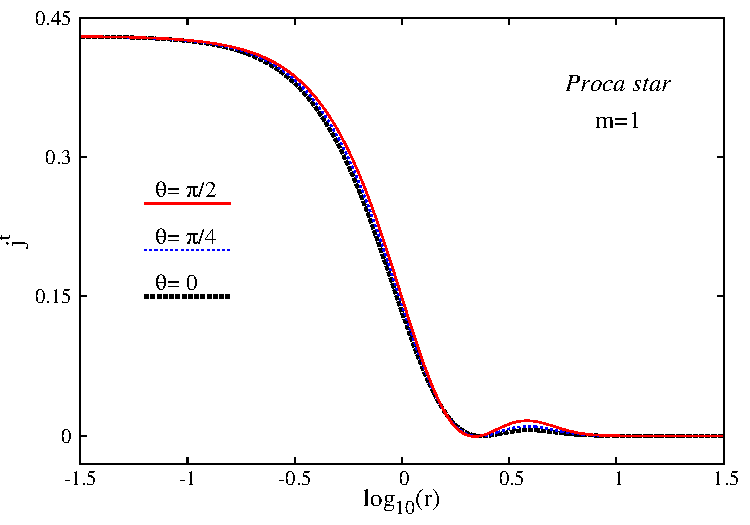
\includegraphics[width=8.1cm]{papers/Proca/PS-jt-m1.pdf}
%       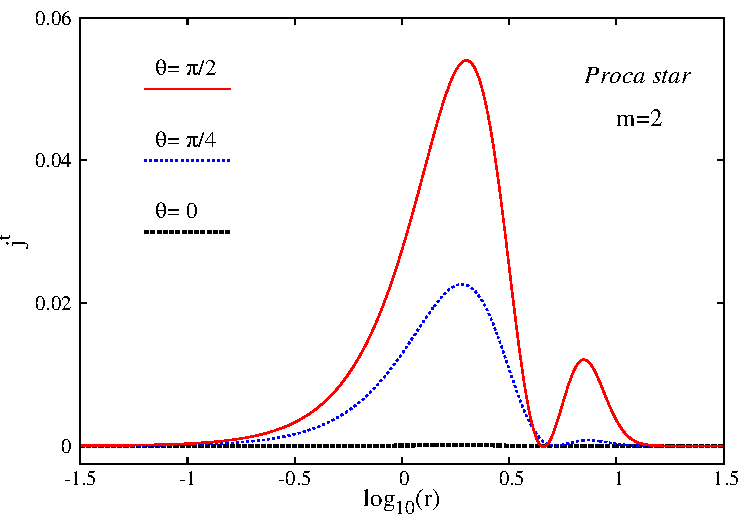
\includegraphics[width=8.1cm]{papers/Proca/PS-jt-m2.pdf}
%   \end{center}
%   \caption{Radial variation of the Noether charge density, $cf.$~\eqref{j}, for different constant $\theta$ sections of the Proca stars exhibited in Fig.~\ref{PS1} (left panel) and Fig.~\ref{PS2} (right panel). One can clearly observe the differences with the angular momentum density.}
%   \label{fignc}
% \end{figure}
% %
% For BHs, on the other hand, there is also a horizon contribution which, in general is non-zero:
% \begin{equation}
% J^{(\mathcal{P})}=mQ+ \oint_\mathcal{H}  P^r dS_r\ .
% \label{JQBHs}
% \end{equation}  
% %%%%%%%%%%%%%%%%%%%%%%%%%%%%%%%%%%%%%%%%%%%%%%%%%
%
%
% This result  contrasts with that for the scalar boson star case, wherein $T_\varphi^t =m j^t $. The total angular momentum and Noether charge, however, are equal in both cases, for stars. This follows from integrating (\ref{s4}) over a spacelike surface and using the Gauss's theorem:
% \begin{eqnarray}
% \label{s6}
% \int T_\varphi^t \sqrt{-g} d^3 x =m \int j^t \sqrt{-g} d^3 x
% + \oint_\infty  P^r dS_r\ .
% \end{eqnarray}
% Since the Proca field decays exponentially, the contribution from the $P^r$ term 
% is zero and one arrives at (\ref{amnc}).
%
%
%
% By using a similar approach, one can easily prove the following identity, where use again the Proca equations (\ref{procafe}) together with
% the expressions 
% $ {\mathcal{F}}_{\alpha t} =\partial_\alpha {\mathcal{A}}_{t}+i w {\mathcal{A}}_{t}$,
% $ \bar{\mathcal{F}}_{\alpha t} =\partial_\alpha \bar{\mathcal{A}}_{t}-i w \bar {\mathcal{A}}_{t}$:
%  \begin{equation}
% \label{sup1}
% T^{\alpha}_\alpha-2T_t^t=
% 2w j^t - \mu^2 {\mathcal{A}}_\alpha \bar{\mathcal{A}}^\alpha+
% \nabla_\alpha U^\alpha,
% \end{equation} 
%  with
% \begin{eqnarray}
% \label{sup2}
%  U^\alpha=\frac{1}{2} 
% \left(
% {\mathcal{A}}_\beta \bar{ {\mathcal{F}}}^{\alpha \beta}+\bar{\mathcal{A}}_\beta { {\mathcal{F}}}^{\alpha \beta}
% \right)
% -\left({\mathcal{A}}_t \bar{ {\mathcal{F}}}^{\alpha t}+\bar{\mathcal{A}}_t { {\mathcal{F}}}^{\alpha t}
% \right)  ~.
% \end{eqnarray}
% For Proca stars,
% the integration of the relation (\ref{sup1}) 
% over a spacelike surface 
% implies the Smarr formula (\ref{smarr-new2}). Here we use again the fact that the Proca field decays exponentially, while the contribution from  $U^r$ at $r=0$ vanishes.
%
% For BHs, however, $U^r$ gives a nontrivial horizon contribution. Then, a combination of (\ref{s4}) and (\ref{sup1}) leads to the simple relation
% \begin{eqnarray}
% \label{sup3}
% \nonumber
% &&T^{\alpha}_\alpha-2T_t^t-2\Omega_H T_\varphi^t =	 2(w-\Omega_H m) j^t - \mu^2 {\mathcal{A}}_\alpha \bar{\mathcal{A}}^\alpha \ \ \ \ \ \ \ \ \ \ \ 
% \\
% &&+
% \frac{1}{\sqrt{-g}}
% \partial_\alpha 
% \bigg[\left(\frac{1}{2} 
% \left(
% {\mathcal{A}}_\beta \bar{ {\mathcal{F}}}^{\alpha \beta}+\bar{\mathcal{A}}_\beta { {\mathcal{F}}}^{\alpha \beta}
% \right)
% -\left(
% ({\mathcal{A}}_t +\Omega_H {\mathcal{A}}_\varphi)\bar{ {\mathcal{F}}}^{\alpha t}
%                 +
% (\bar{\mathcal{A}}_t +\Omega_H \bar{\mathcal{A}}_\varphi){ {\mathcal{F}}}^{\alpha t}
% \right)
% \right)  
% \sqrt{-g} 
% \bigg] \ .
% \end{eqnarray}
% The integration of this identity leads to the simplified 
% Smarr formula (\ref{smarr-new1}). Here one uses also the synchronization 
% condition (\ref{synchronization}), 
% together with  the boundary conditions (\ref{bccloudshorizon}).  
